\begin{figure}[h]
\centering
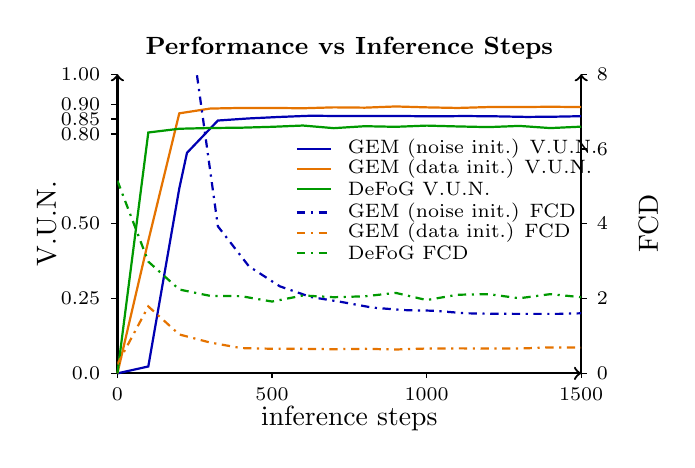
\begin{tikzpicture}[scale=0.95]
  \draw[->, thick] (0,0) -- (6.2,0) node[midway, below=8pt] {inference steps};
  \draw[->, thick] (0,0) -- (0,4.0);
  \node[rotate=90] at (-0.95,2.0) {V.U.N.};
  \draw[->, thick] (6.2,0) -- (6.2,4.0);
  \node[rotate=90] at (7.1,2.0) {FCD};

  % Title
  \node[font=\small\bfseries] at (3.1,4.35) {Performance vs Inference Steps};

  % Axes ticks
  \foreach \x/\lab in {0/0,2.067/500,4.133/1000,6.200/1500} {
    \draw (\x,0) -- (\x,-0.06);
    \node[below, font=\scriptsize] at (\x,-0.06) {\lab};
  }
  \foreach \y/\lab in {0/0.0,1.0/0.25,2.0/0.50,3.2/0.80,3.4/0.85,3.6/0.90,4.0/1.00} {
    \draw (0,\y) -- (-0.08,\y);
    \node[left, font=\scriptsize] at (-0.1,\y) {\lab};
  }
  \foreach \y/\lab in {0/0,1.0/2,2.0/4,3.0/6,4.0/8} {
    \draw (6.2,\y) -- (6.28,\y);
    \node[right, font=\scriptsize] at (6.28,\y) {\lab};
  }
  % Noise initialization (warmup + DLangevin)
  \draw[blue!70!black, thick] plot coordinates {
    (0.000,0.000) (0.413,0.092) (0.827,2.472) (0.930,2.948) (1.343,3.380)
    (1.757,3.408) (2.170,3.428) (2.583,3.444) (2.997,3.440) (3.410,3.440)
    (3.823,3.440) (4.237,3.436) (4.650,3.440) (5.063,3.436) (5.477,3.428)
    (5.890,3.432) (6.200,3.438)
  };

  % Data initialization (annealed)
  \draw[orange!90!black, thick] plot coordinates {
    (0.000,0.000) (0.413,1.772) (0.827,3.476) (1.240,3.540) (1.653,3.548)
    (2.067,3.548) (2.480,3.544) (2.893,3.556) (3.307,3.552) (3.720,3.568)
    (4.133,3.556) (4.547,3.548) (4.960,3.560) (5.373,3.560) (5.787,3.564)
    (6.200,3.560)
  };

  % DeFoG
  \draw[green!60!black, thick] plot coordinates {
    (0.000,0.000) (0.413,3.220) (0.827,3.270) (1.240,3.280) (1.653,3.284)
    (2.067,3.296) (2.480,3.313) (2.893,3.278) (3.307,3.304) (3.720,3.296)
    (4.133,3.312) (4.547,3.301) (4.960,3.292) (5.373,3.308) (5.787,3.279)
    (6.200,3.298)
  };

  % FCD (right axis)
  \begin{scope}
    \clip (0,0) rectangle (6.2,4.0);
    \draw[blue!70!black, thick, dash dot] plot coordinates {
      (0.413,8.184) (0.827,4.961) (0.930,4.952) (1.343,1.966) (1.757,1.432)
      (2.170,1.164) (2.583,1.021) (2.997,0.954) (3.410,0.879) (3.823,0.846)
      (4.237,0.837) (4.650,0.803) (5.063,0.796) (5.477,0.795) (5.890,0.795)
      (6.200,0.803)
    };
    \draw[orange!90!black, thick, dash dot] plot coordinates {
      (0.000,0.122) (0.413,0.895) (0.827,0.520) (1.240,0.412) (1.653,0.338)
      (2.067,0.329) (2.480,0.328) (2.893,0.323) (3.307,0.328) (3.720,0.319)
      (4.133,0.332) (4.547,0.334) (4.960,0.333) (5.373,0.332) (5.787,0.347)
      (6.200,0.344)
    };
    \draw[green!60!black, thick, dash dot] plot coordinates {
      (0.000,2.575) (0.413,1.494) (0.827,1.121) (1.240,1.036) (1.653,1.032)
      (2.067,0.960) (2.480,1.041) (2.893,1.018) (3.307,1.030) (3.720,1.076)
      (4.133,0.980) (4.547,1.051) (4.960,1.059) (5.373,1.004) (5.787,1.059)
      (6.200,1.018)
    };
  \end{scope}

  % Legend
  \begin{scope}[shift={(2.25,1.35)}]
    \draw[blue!70!black, thick] (0.15,1.65) -- (0.6,1.65);
    \node[anchor=west, font=\scriptsize] at (0.7,1.65) {GEM (noise init.) V.U.N.};
    \draw[orange!90!black, thick] (0.15,1.38) -- (0.6,1.38);
    \node[anchor=west, font=\scriptsize] at (0.7,1.38) {GEM (data init.) V.U.N.};
    \draw[green!60!black, thick] (0.15,1.11) -- (0.6,1.11);
    \node[anchor=west, font=\scriptsize] at (0.7,1.11) {DeFoG V.U.N.};
    \draw[blue!70!black, thick, dash dot] (0.15,0.80) -- (0.6,0.80);
    \node[anchor=west, font=\scriptsize] at (0.7,0.80) {GEM (noise init.) FCD};
    \draw[orange!90!black, thick, dash dot] (0.15,0.53) -- (0.6,0.53);
    \node[anchor=west, font=\scriptsize] at (0.7,0.53) {GEM (data init.) FCD};
    \draw[green!60!black, thick, dash dot] (0.15,0.26) -- (0.6,0.26);
    \node[anchor=west, font=\scriptsize] at (0.7,0.26) {DeFoG FCD};
  \end{scope}
\end{tikzpicture}
\caption{\footnotesize \textbf{V.U.N. and FCD vs Steps.} V.U.N. (higher is better) and FCD (lower is better) versus inference steps on MOSES for GEM noise initialization (uniform) with greedy warmup proposal, GEM data initialization with annealed proposal, and DeFoG (marginal noise).}
\label{fig:moses-vun-steps}
\end{figure}
